%\VignetteIndexEntry{MHDE Package}

\documentclass{article}
\usepackage{tabulary}
\usepackage{graphicx}
\usepackage[style=authoryear-comp, maxnames=1, bibencoding=utf8, backend=biber]{biblatex}
\bibliography{mhde.bib}


\title{mhde: An R Package for a Goodness-of-Fit Test for Normality Using the Minimum Hellinger Distance }

\usepackage{Sweave}
\begin{document}
\Sconcordance{concordance:mhde_article.tex:mhde_article.Rnw:%
1 11 1 1 0 124 1 1 4 3 0 1 1 3 0 1 2 2 1 1 7 6 0 1 1 3 0 1 2 41 1}



\section{Goodness-of-Fit Test for Normality Using the Minimum Hellinger Distance}
Statistical data analysis techniques rest on assumptions about the form of the data.  Some techniques are sensitive to small deviations from the assumptions while others are more robust.  Unfortunately, robust techniques are not usually optimal when the data follow the true model.  However, one robust estimator \parencite{beran1977a} \parencite{beran1977b} based on the minimum Hellinger distance between a parametric family of densities and a nonparametric density estimator (called the mhde) is also asymptotically efficient \parencite{stather1981}.  The minimized Hellinger distance can also be used in a goodness-of-fit test for the parametric family \parencite{beran1977a}.

Empirically based critical values for a goodness-of-fit test for normality based on the Hellinger distance were developed \parencite{eslinger1991} using a limited number of simulations and they are not readily accessible to the general community of practitioners.  This paper updates and expands the critical values for the minimum Hellinger distance goodness-of-fit test for normality and introduces the mhde R package \parencite{mhde}.  The package determines the mean and standard deviation of the normal distribution that minimizes the Hellinger distance and calculates the p-value for a goodness-of-fit test.

\section{Statistical methods}

Let $f(x)$ and $g(x)$ be absolutely continuous functions.  The square of the Hellinger distance \parencite{hellinger1909} is defined as:

\begin{equation}
\label{eq:Hellinger_Distance}
H^2 = \frac{1}{2} \int(f^{1/2}(x) - g^{1/2}(x))^2dx
\end{equation}

Some authors omit the $\frac{1}{2}$ term in the distance definition, but we include it.  For purposes of this paper, $f$ and $g$ are constrained to be  probability density functions that integrate to $1$ by definition.  Using this constraint, one can expand the square in the integral and obtain the following alternative form:

\begin{equation}
\label{eq:Hellinger_Modified}
H^2 = 1 - \int\sqrt{f(x)g(x)}dx
\end{equation}

The Hellinger distance is the integral of a non-negative function and it reaches the minimum value of 0 when $f$ and $g$ are identical.  The expanded form in Equation \ref{eq:Hellinger_Modified} shows it can take on a maximum value of 1 when $f$ and $g$ are mutually singular.

For this paper, $f$ denotes the family of normal densities.  Thus,

\begin{equation}
\label{eq:f_density}
f(x) = \frac{1}{\sigma\sqrt{2\pi}}e^{-(\frac{x - \mu}{\sigma})^2}
\end{equation}

for $-\infty\leq\mu\leq\infty$ and $\sigma>0$.  The goodness-of-fit test uses a null hypothesis that the data come a normal distribution without specifying the mean and standard deviation.  The minimum Hellinger distance approach can be used with any parametric family of distributions, but the mhde R package only contains routines and p values for the family of normal densities.

\subsection{Sample density fitting using the Epanechnikov kernel}

This implementation defines $g$ as the data-based density obtained by using the Ephanechnikov kernel \parencite{epanechnikov1969}.  The kernel has the form $w(z)=0.75(1-z^2 )$ for $-1<z<1$ and 0 elsewhere.  Let the $n$ sample data be denoted by $x_1, ..., x_n$.  The data-based kernel density at any point $y$ is calculated from

\begin{equation}
\label{eq:g_density}
g_n(y) = \frac{1}{nh_n}\sum\limits_{i=1}^n w(\frac{y-x_i}{h_n})
\end{equation}

The term $h_n$ is a constant at any specific sample size.  The sequence of $h_n$ terms must converge to zero as the sample size goes to $\infty$.  An optimal form for $h_n$ is available \parencite{schucany1977} when estimating the mean value of the normal distribution, but the resulting sequence leads to biased scale estimates.

It is useful to treat $h_n$ as the product of a scale value, $s_n$, and a constant, $c_n$.  The scale value, $s_n$, can be approximated by the sample median absolute deviation.  Location estimates for normal models are relatively insensitive to the choice of $c_n$, while scale estimates are quite sensitive to the choice of $c_n$.  The $c_n$ sequence in the mhde R package was chosen to yield unbiased scale estimates for the normal family of densities.  As a benefit, the location estimates are also unbiased.  Initial empirical studies \parencite{eslinger1991} used 5000 replications at 15 sample sizes in the 20 to 1000 range to obtain the functional form $c_n=2.283n^{-0.287}$.  Unfortunately, this simple sequence leads to biased scale estimates for sample sizes smaller than about 20.

An expanded empirical study used 276 different sample sizes ranging from 5 to 10,000 to determine the optimal $c_n$ sequence.  Six replications were performed at each sample size.  Each replication used a Gauss-Newton iterative approach to pick the $c_n$ to yield the unbiased scale estimate based on $10^6$ samples.  Specific values for $c_n$ use the average of the six replicates for samples sizes from 5 to 40.  Larger sample sizes all use a fit of the form $c_n=a\times n^b$ but the sample sizes are divided into 17 subsets.  The functional fits within each subset pass lack of fitness tests and the largest residuals within subsets are smaller than 0.1\% of the nominal $c_n$.  Explicit values of $c_n$ are not provided in the text, but the \textbf{mhde.cn} function in the R package can be used to retrieve the $c_n$ value for any sample size.

\subsection{Critical values}

The previous published limited set of critical values \parencite{eslinger1991} use the form of Equation \ref{eq:Hellinger_Distance} without the $\frac{1}{2}$ term and are not valid for the new $c_n$ sequence.  New critical values, $m_c$, for a goodness-of-fit test for normality were derived empirically using the new $c_n$ sequence.  The percentiles of the distribution when the data are normally distributed were calculated at 63 different levels from 0.0001 to 0.9999 using 12 replicates of $10^6$ data sets at 276 sample sizes from 5 to 10,000.  The large number of data sets provides stable percentiles in the tails of the distribution.

The $m_c$ values use the average of replicates for samples sizes from 5 to 40.  Larger sizes all use a fit of the form $m_c=a\times n^b$ where the sample sizes are broken into 18 separate groups. For $n$ larger than 8000, the functional form is $c_n=2.4130 n^{-0.29332}$, thus the sequence does converge to $0$ for large samples sizes.  Explicit values of $m_c$ are not provided in the text, but the \textbf{mhde.crit} function in the R package can be used to retrieve the $m_c$ for any sample size and desired $\alpha$ level.

The implementation in the mhde R package uses two steps for generating p-values for the test for normality.  First, a vector of $m_c$ values for all 63 percentiles is generated for the specific sample size.  Second, the p-value is calculated using linear interpolation among the 63 percentiles given the minimized distance for a specific data set.

Large values of the minimized Hellinger distance indicate a poor match between the nonparametric data-based density estimate and the normal family of densities.  Thus, a one-tailed statistical test is appropriate.

\subsection{Power of the test}

A number of authors, \parencite{razali2011} for example, have studied the statistical power of tests for normality against a wide range of alternative distributions.  Five of the most commonly used tests for normality are available in the nortest R package \parencite{gross2015}.  The Shapiro-Wilks test \parencite{shapiro1965} generally has the highest power of any of the common tests for normality, therefore, the power of the mhde test is compared to the power of the Shapiro-Wilks test for eight distributions.  The power of the tests is provided in Table \ref{tab:power_vals} for an $\alpha=0.05$ significance level using  $10^5$ replications.  The uniform and triangular distributions are symmetric and shorter tailed than the normal distribution.  The Cauchy, Student's t(2) and Student's t(4) are symmetric and longer tailed than the normal distribution.  The Weibull (2), exponential and Chi-Square (1) distributions are skewed.  Results for the normal distribution are provided to show the appropriateness of the critical values.

\begin{table}[h!]
\begin{tabular}{ll*{10}{c}}
\hline
\textbf{Distribution} & \textbf{Test} & \textbf{10} & \textbf{20} & \textbf{30} & \textbf{40} & \textbf{50} & \textbf{60} & \textbf{80} & \textbf{100} \\
\hline
\textbf{Normal} & mhde & 0.043 & 0.048 & 0.050 & 0.049 & 0.051 & 0.049 & 0.050 & 0.050\\
 & shapiro & 0.047 & 0.050 & 0.051 & 0.049 & 0.051 & 0.049  & 0.049 & 0.049\\
\textbf{Cauchy} & mhde & 0.499 & 0.851 & 0.956 & 0.988 & 0.996 & 0.999  & 0.999  & 0.999\\
 & shapiro & 0.591 & 0.866 & 0.958 & 0.988 & 0.996 & 0.999 & 1.000 & 1.000\\
\textbf{Chi Square (1)} & mhde & 0.552 & 0.920 & 0.991 & 1.000 & 1.000 & 1.000  & 1.000  & 1.000\\
 & shapiro & 0.739 & 0.984 & 1.000 & 1.000 & 1.000 & 1.000  & 1.000  & 1.000\\
\textbf{Exponential} & mhde & 0.273 & 0.655 & 0.889 & 0.975 & 0.996 & 1.000 & 1.000 & 1.000\\
 & shapiro & 0.446 & 0.836 & 0.968 & 0.995 & 0.999 & 1.000  & 1.000  & 1.000\\
\textbf{Student's t (2)} & mhde & 0.222 & 0.480 & 0.651 & 0.767 & 0.842 & 0.896 & 0.954 & 0.980\\
 & shapiro & 0.296 & 0.529 & 0.684 & 0.793 & 0.864 & 0.911 & 0.963 & 0.985\\
\textbf{Student's t (4)} & mhde & 0.106 & 0.205 & 0.287 & 0.357 & 0.416 & 0.470  & 0.561  & 0.634\\
 & shapiro & 0.138 & 0.240 & 0.326 & 0.403 & 0.467 & 0.526 & 0.627  & 0.708\\
\textbf{Triangular} & mhde & 0.014 & 0.012 & 0.013 & 0.016 & 0.022 & 0.030 & 0.057  & 0.101\\
 & shapiro & 0.029 & 0.034 & 0.040 & 0.049 & 0.058 & 0.069 & 0.095 & 0.132\\
\textbf{Uniform} & mhde & 0.026 & 0.036 & 0.076 & 0.206 & 0.562 & 0.900 & 1.000  & 1.000\\
 & shapiro & 0.131 & 0.453 & 0.816 & 0.979 & 0.999 & 1.000 & 1.000 & 1.000\\
\textbf{Weibull (2)} & mhde & 0.042 & 0.075 & 0.129 & 0.197 & 0.280 & 0.370 & 0.555 & 0.716\\
 & shapiro & 0.074 & 0.147 & 0.234 & 0.325 & 0.419 & 0.509 & 0.671  & 0.796\\
\hline
\end{tabular}
\caption{Statistical power of the mhde and Shapiro-Wilks tests for normality for different sample sizes using eight distributions and an $\alpha=0.05$ significance level.}
\label{tab:power_vals}
\end{table}

The mhde test is generally less powerful than the Shapiro-Wilks test.  However, in some situations the mhde test is competitive with or more powerful than the Shapiro-Wilks test.  For example, neither test is very powerful for the alternative triangular distribution for small sample sizes.  The power of the mhde test is compared with the power of the Shapiro-Wilks test for a symmetric triangular distribution in Figure \ref{fig:power} for larger sample sizes.

\begin{figure}[h!]
\centering
%%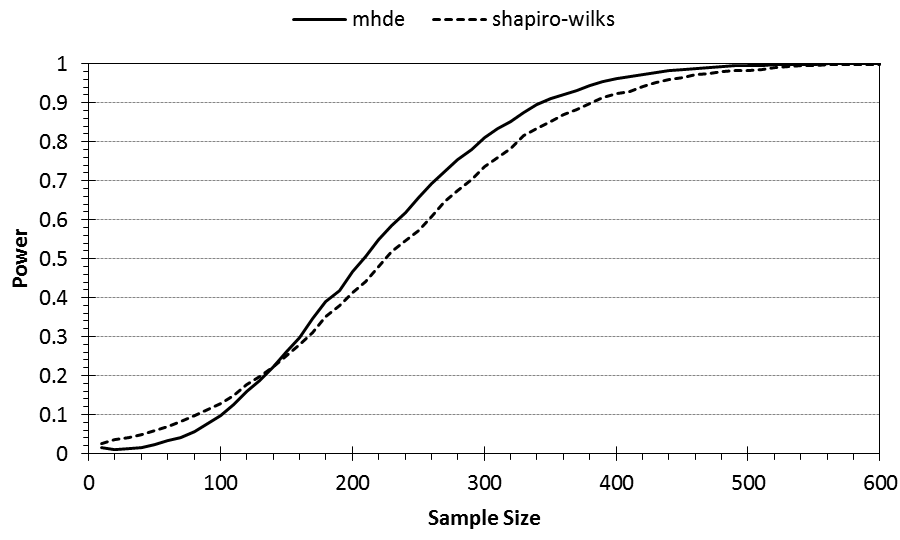
\includegraphics[width=\textwidth,natwidth=943,natheight=635]{power.png}
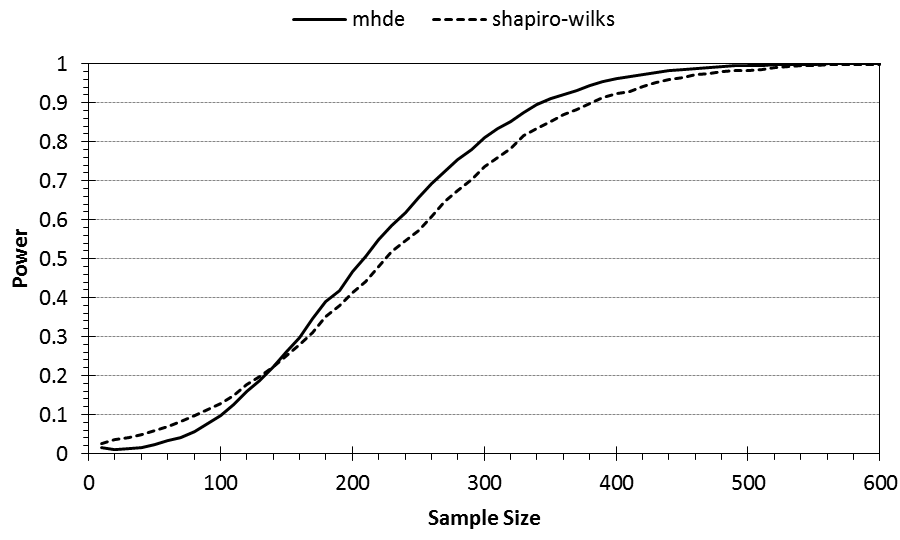
\includegraphics[scale=1.0]{power.png}
\caption{Power of the mhde and Shapiro-Wilks tests for the alternative of a symmetric triangular distribution using an $\alpha=0.05$ significance level.}
\label{fig:power}
\end{figure}

\section{Package architecture and implementation details}

The mhde package for the R environment for statistical computing and graphics \parencite{rcore2015} can be downloaded from the Comprehensive R Archive Network (CRAN) \parencite{cran}.  The package fits a minimum Hellinger distance model to sample data and performs a goodness-of-fit test for normality. The primary function in the mhde package is \textbf{mhde.test}. Three utility functions are also provided.  The function \textbf{mhde.cn} returns the value of $c_n$ for a single sample size.  The function \textbf{mhde.crit} returns the critical value for a given sample size and desired (lower-tail) probability level.  The function \textbf{mhde.plot} generates a plot of the kernel density and optimized normal density using output from the function \textbf{mhde.test}.

\subsection{Solution techniques}

Calculating the Hellinger distance requires numerical evaluation of the integral in Equation \ref{eq:Hellinger_Modified}.  The integral is evaluated using a composite Gauss-Legendre 6-point integration scheme \parencite{beyer1987}.  The implementation defaults to 100 subintervals, resulting in about 5 digits of accuracy in the location and scale estimate.  The user can specify 25 or more subintervals.

Maximization of the integral in Equation \ref{eq:Hellinger_Modified} is performed simultaneously for location ($\mu$) and scale ($\sigma$) using an iterative Gauss-Newton technique with analytical derivatives.  The default location starting value is the sample median and the default scale starting value is the sample median absolute deviation.  If the procedure initially fails to converge, Hellinger distances are evaluated on a 21 by 21 grid of location and scale values spread across a range of reasonable values for the specific data set.  The ($\mu$,$\sigma$) point on the grid with the associated minimum Hellinger distance is used to restart the iterative technique.  If the iterative technique still does not converge, the returned solution is the best fit in the grid search.  The authors have not encountered any data sets where the procedure failed to converge after invoking the grid search procedure.

\subsection{Accuracy and limitations}
Convergence of the iterative technique is declared when an update step results in small changes in both the location and scale values.  The user can specify the epsilon (in data units) for convergence.  Both location (\textbf{EpsLoc}) and scale (\textbf{EpsSca}) epsilons should be set to give approximately 4 to 5 digits of accuracy in the estimates.  Default values of 0.0001 are used for both location and scale.  These values are appropriate if the data are normally distributed with a mean near 0 and a scale of 1.

The critical values of the test were derived empirically.  Values in the extreme tails of the distribution are difficult to determine accurately.  Therefore, critical values for percentiles greater than 0.9999 are set to the critical value for 0.9999 and critical values for percentiles less than 0.0001 are set to the critical value for 0.0001.  Similarly, p-values are constrained to the 0.0001 to 0.9999 range.  These limitations have no practical significance because statistical tests are rarely performed for $\alpha$ levels outside 0.9 to 0.99.

\subsection{Example usage}

The function \textbf{mhde.test} returns a list of objects.  The objects are the minimized Hellinger distance, the p-value for the test, the initial location and scale for the iterative solution, the final location and scale, the sample size, the value for $c_n$, and three vectors.  The first vector contains the $X$ values (in the sample domain) used in the numerical integration.  The final two vectors contain the kernel density function and the best fit normal density at the $X$ values.

The following example use of the function \textbf{mhde.test} uses a sample of 10 data values from a normal distribution.  This example does not converge using the initial values, but it does converge using the values from the internal grid search.  The p value of 0.148 does not lead to rejection of the null hypothesis that the data came from a normal distribution.

\begin{Schunk}
\begin{Sinput}
> MyData <- c(0.70881649,0.56886754,0.85748977,0.77956422,
+ -0.40878175,-0.06055631,0.57249616,0.06287769,
+ 0.62590278,-0.26852515)
> Out <- mhde.test(MyData)
\end{Sinput}
\end{Schunk}

The following example uses a sample of 25 data values from a Student's t(2) distribution.  This distribution has longer tails than the normal distribution and the small p value of 0.0083 leads to rejection of the null hypothesis that the data came from a normal distribution.

\begin{Schunk}
\begin{Sinput}
> MyData <- c(0.28278713,-0.43277345,-0.44767540,-0.81732116,
+ +   -0.84096097,0.04163228,1.94541307,-1.09498962,0.96905752,
+ +   -0.08427381,0.11302093,-9.35078076,0.01315122,0.39547341,
+ +   -0.33285223,0.05248393,1.50556785,-1.22518816,0.80181014,
+ +   -0.02247526,3.48830616,0.47796627,-0.21144776,-3.14836990,
+ +   -1.74839250)
> Out <- mhde.test(MyData)
\end{Sinput}
\end{Schunk}

A simple plot of the normal and kernel densities can be generated using the function \textbf{mhde.plot} with the list returned from the function \textbf{mhde.test} as the argument.  Example plots of the normal and kernel densities used in the two example cases are provided in Figure 2.  The nonparametric density for small data sets with long tails can have multiple modes separated by regions where the density is zero.

\begin{figure}[h]
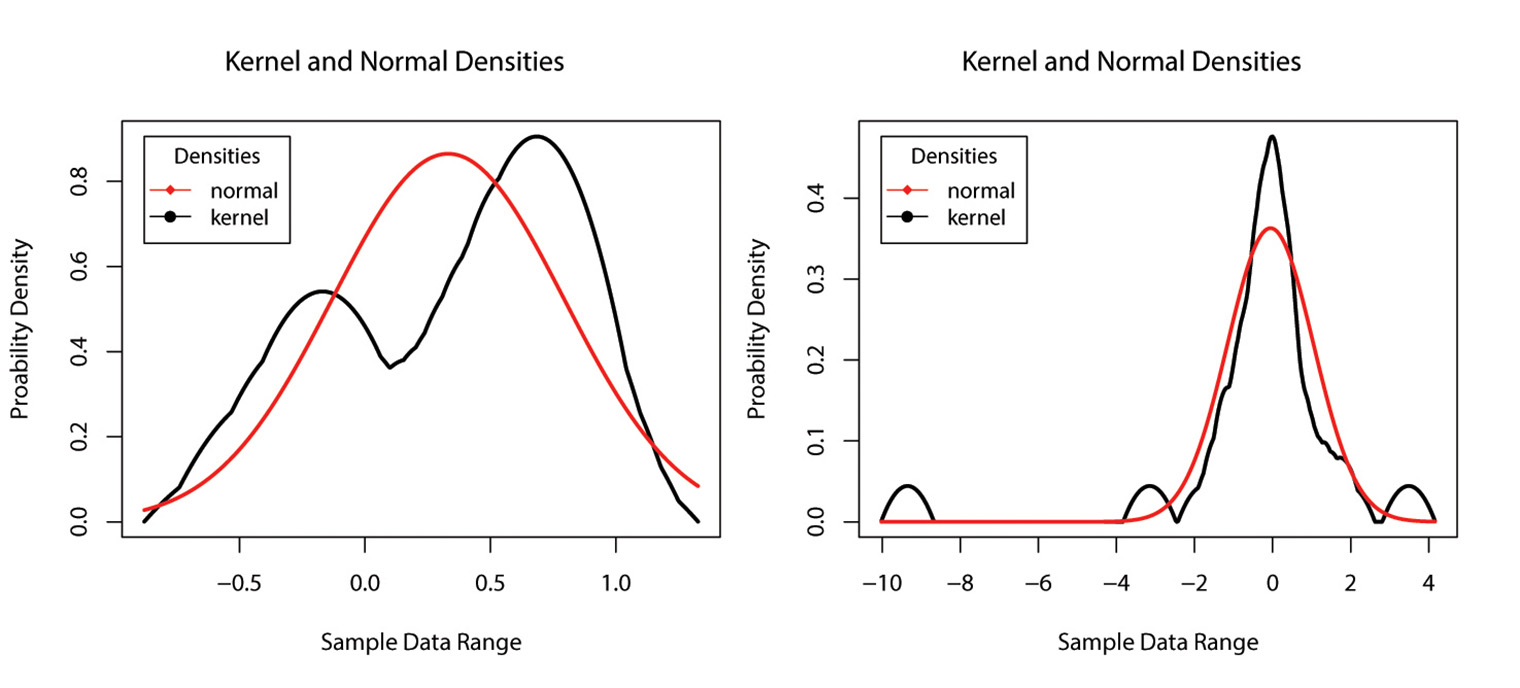
\includegraphics[width=\textwidth]{density_plots.jpg}
\caption{Plot of the normal and kernel densities used in the example cases of 10 data points (left pane) and 25 data points (right pane).}
\label{fig:mhde.plot}
\end{figure}

\begin{tabulary}{\textwidth}{p{2.1cm}L}
\multicolumn{2}{l}{The function \textbf{mhde.test} has the following arguments:}\\
\textbf{DataVec} & The data are supplied in the numeric vector \textbf{DataVec}.  The length of the vector determines the number of data values.  There is no default value.\\
\textbf{NGauss} & The number of subintervals for the Gauss-Legendre integration techniques is controlled by \textbf{NGauss}.  A default value of 100 is used.  A minimum of 25 is enforced.\\
\textbf{MaxIter} & The maximum number of iterations used for evaluating the minimum Hellinger distance is controlled by \textbf{MaxIter}.  A default of 25 is used.  A minimum of 1 is enforced.\\
\textbf{InitLocation} & An optional initial location estimate can be defined using \textbf{InitLocation}.  The data median is the default value.\\
\textbf{InitScale} & An optional initial scale estimate can be defined using \textbf{InitScale}.  The median absolute deviation of the data is the default value.\\
\textbf{EpsLoc} & The epsilon (in data units) below which the iterative minimization approach declares convergence in the location estimate is controlled by \textbf{EpsLoc}.  \textbf{EpsLoc} should be set to give approximately 5 digits of accuracy in the location estimate.  A default value of 0.0001 is used.\\
\textbf{EpsSca} & The epsilon (in data units) below which the iterative minimization approach declares convergence in the scale estimate is controlled by \textbf{EpsSca}.  \textbf{EpsSca} should be set to give approximately 5 digits of accuracy in the scale estimate.  A default value of 0.0001 is used.\\
\textbf{Silent} & By default \textbf{mhde.test} writes several results to the R console.  Use \textbf{Silent}=TRUE to eliminate the output.\\
\textbf{Small} & By default \textbf{mhde.test} returns a list of 10 objects.  Use \textbf{Small}=TRUE to return a shorter list consisting only of the minimized Hellinger distance and the p-value of the goodness-of-fit test.
\end{tabulary}

\begin{tabulary}{\textwidth}{p{2cm}L}
\multicolumn{2}{l}{The function \textbf{mhde.cn} has the following arguments:}\\
\textbf{Nsize} & The sample size is defined using \textbf{Nsize}.  No default value is set.\\
\\
\multicolumn{2}{l}{The function \textbf{mhde.crit} has the following arguments:}\\
\textbf{Nsize} & The sample size is defined using \textbf{Nsize}.  No default value is set.\\
\textbf{Plevel} & The probability level associated with the critical value is set using \textbf{Plevel}.  A default value of 0.95 is used.  The $\alpha$ level of the test is 1-\textbf{Plevel}.\\
\\
\multicolumn{2}{l}{The function \textbf{mhde.plot} has the following arguments:}\\
\textbf{ListOut} & The list of objects returned by \textbf{mhde.test} is provided in \textbf{ListOut}.  The argument \textbf{Small} for \textbf{mhde.test} must have the value FALSE.\\
\end{tabulary}

\section{Discussion}

In this article we present the mhde package for fitting a normal model to data using a minimum Hellinger distance estimator and performing a goodness-of-fit test for normality.  The package improves previously published critical values and makes the mhde estimator available to the statistical computing community.

\printbibliography


\end{document}
